
\documentclass{article}
\usepackage[utf8]{inputenc}
\usepackage{graphicx}
\usepackage{amsmath}
\usepackage{hyperref}
\usepackage{float}
\usepackage{geometry}
\usepackage{titling}
\usepackage{amssymb}
\usepackage{abstract}
\usepackage{multicol}
\usepackage{biblatex}
\usepackage{listings} % Add the missing LaTeX package
\usepackage{subcaption}



% \usepackage{quantikz}


\addbibresource{bibliography.bib}
\geometry{a4paper, left=2cm, right=2cm, top=2cm, bottom=2cm}


\usepackage{fancyhdr}

\pagestyle{fancy}
\fancyhf{}
\lhead{M1 PAD \\ \rule{\textwidth}{0.4pt} \\ M1 Project}
\rhead{MU4PYD? \\ \rule{\textwidth}{0.4pt} \\ 2023-2024}
\renewcommand{\headrulewidth}{0pt}

\begin{document}

\title{M1 Project - Quantum Optimization}
\author{Martin PUJOL \\ martin.pujol@etu.sorbonne-universite.fr}
\date{}

\maketitle
\thispagestyle{fancy}


\begin{abstract}

This bibliographic project aims to briefly introduce the foundational principles of quantum computing, address the concept of a qubit, ways to produce them, and the challenges associated with their usage. Subsequently, the project takes a more hands-on approach by formalizing a (simplistic) optimization problem and solving it using a quantum computer.

\textbf{Keywords: Quantum Computing, Qubit, Optimization}

\end{abstract}

\begin{multicols}{2}

\section{What is a qubit?}
\subsection{Definition}

A qubit, short for "quantum bit" is the basic unit of quantum computing. From a physicist's perspective, it can simply be considered as a two-level quantum system. A qubit is a quantum system that can exist in two basis states, denoted as $\left|0\right>$ and $\left|1\right>$. To define the state of this qubit, we need two complex numbers \( a \) and \( b \) such that \( a^2 + b^2 = 1 \). We can write the state of the qubit as follows:
\begin{equation}
\left|\psi\right> = a\left|0\right> + b\left|1\right>
\end{equation}

This is commonly represented as a column vector:

\begin{equation}
\left|\psi\right> = \begin{pmatrix} a \\ b \end{pmatrix}
\end{equation}

It is illustrated on the Bloch sphere:

\begin{figure}[H]
    \centering
    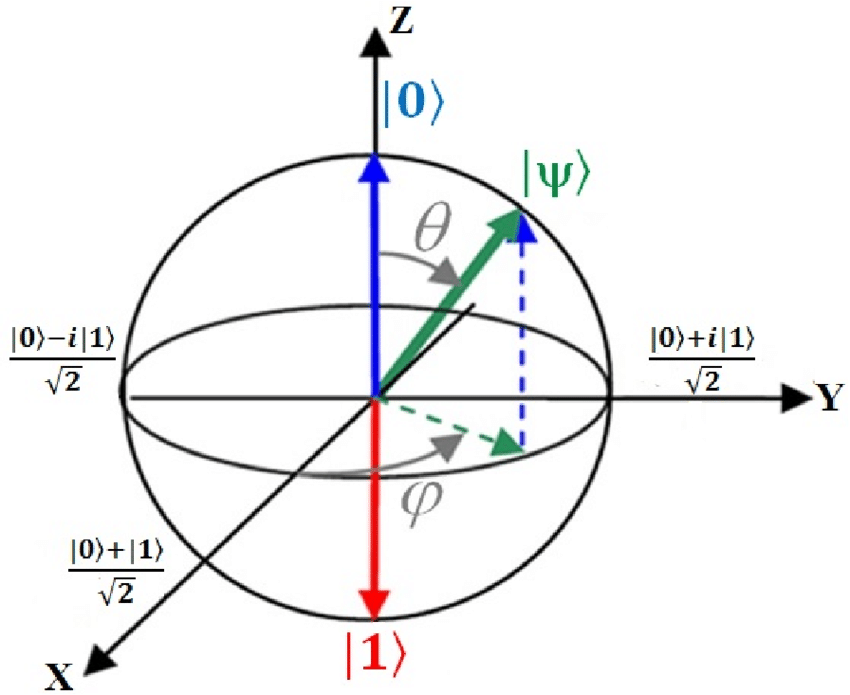
\includegraphics[width = \columnwidth]{fig/bloch_sphere.png}
    \caption{Bloch Sphere}
    \label{fig:sphere_de_bloch}
\end{figure}



Since a quantum state is defined up to a global phase factor, we can ensure that \( a \) is real. This property allows us to represent the state of a qubit in three dimensions. Adding the constraint on its norm enables us to visualize this state on the Bloch sphere (see Figure \autoref{fig:sphere_de_bloch}).

\subsection{Measuring a qubit}

Measuring a qubit is somewhat unique because it destroys the superposition. Measurement is an irreversible process that projects the state of the qubit onto one of its two basis states. We define two projection operators, $\left|0\right>\left<0\right|$ and $\left|1\right>\left<1\right|$. The probability of measuring the state $\left|0\right>$ is given as follows:

\begin{equation}
    P(\left|0\right>) = \left<\psi\right|\left|0\right>\left<0\right|\left|\psi\right> = a^2
\end{equation}

And the probability of measuring the state $\left|1\right>$ is given as follows:

\begin{equation}
    P(\left|1\right>) = \left<\psi\right|\left|1\right>\left<1\right|\left|\psi\right> = b^2
\end{equation}

It becomes evident that we cannot measure the state of our qubit during computation. The challenge lies in exploiting the quantum properties of the qubit without measuring it. Only at the end of these manipulations can we measure the qubit to obtain the result using, among others, the projection operators defined earlier.

\subsection{Superposition and entanglement of qubits}

Introducing the notion of a qubit may not immediately reveal how computational power can be harnessed from such a system. By analogy with classical bits, we can consider what happens when using \( N \) qubits. This results in a quantum system with \( 2^N \) basis states, allowing the system to exist in a superposition of \( 2^N \) different states. For instance, the state of a 3-qubit system can be written as:

\begin{align}
    \left|\psi\right> = & a\left|000\right> + b\left|001\right> + c\left|010\right> \nonumber \\
    & + d\left|011\right> + e\left|100\right> + f\left|101\right> \nonumber \\
    & + g\left|110\right> + h\left|111\right>
\end{align}

Represented as a column vector:

\begin{equation}
    \left|\psi\right> = \begin{pmatrix} a \\ b \\ c \\ d \\ e \\ f \\ g \\ h \end{pmatrix}
\end{equation}

Thus, three qubits carry information of size \( 2^3 = 8 \) continuous variables.

Superposition is particularly interesting because it allows us to "explore" various superposed states to find the solution to an optimization problem. This extensive superposition space enables compact information encoding and computation by carefully preparing and measuring states.

Entanglement introduces a useful concept that allows the creation of correlations between states, enabling the transmission of information from one state to another. Quantum states can be prepared in such a way that they cannot be described as a superposition of two independent quantum states. For example, Bell states are:ntanglement introduces a useful concept that allows the creation of correlations between states, enabling the transmission of information from one state to another. Quantum states can be prepared in such a way that they cannot be described as a superposition of two independent quantum states. For example, Bell states are:

\begin{equation}
    \left|\psi\right> = \frac{1}{\sqrt{2}}\left(\left|00\right> + \left|11\right>\right)
\end{equation}

\begin{equation}
    \left|\psi\right> = \frac{1}{\sqrt{2}}\left(\left|00\right> - \left|11\right>\right)
\end{equation}

\begin{equation}
    \left|\psi\right> = \frac{1}{\sqrt{2}}\left(\left|01\right> + \left|10\right>\right)
\end{equation}

\begin{equation}
    \left|\psi\right> = \frac{1}{\sqrt{2}}\left(\left|01\right> - \left|10\right>\right)
\end{equation}

For these states, measuring one qubit immediately reveals the state of the other qubit. 

At this stage, the idea of quantum computation might still seem abstract, especially for the author! Fortunately, after discussing how to produce qubits, we will encode an optimization problem and solve it using a quantum computer.

\section{How to produce a qubit and manipulate its state?}

Since a qubit is a two-level quantum system, it can be realized using a variety of physical systems. These include atoms, ions, photons, spin defects, quantum dots, molecules, superconductors, and more. It is challenging to be exhaustive here, but both industry and research focus on a few promising technologies. These technologies, which we will concentrate on, include superconducting qubits, trapped-ion qubits, and photonic qubits. 

These technologies are promising for several reasons: a qubit needs to be highly stable (maintaining its state as long as possible), scalable (easy to produce and manipulate in large numbers), and enable certain quantum properties such as entanglement.

\subsection{Trapped-ion qubits}

Trapped-ion qubits consist of hydrogen-like ions trapped in an electromagnetic field. The quantum system to consider here is the energy level of the ion’s electron. The ions are first cooled to temperatures near absolute zero and then trapped in a quadrupole electromagnetic field, as shown below:

\begin{figure}[H]
    \centering
    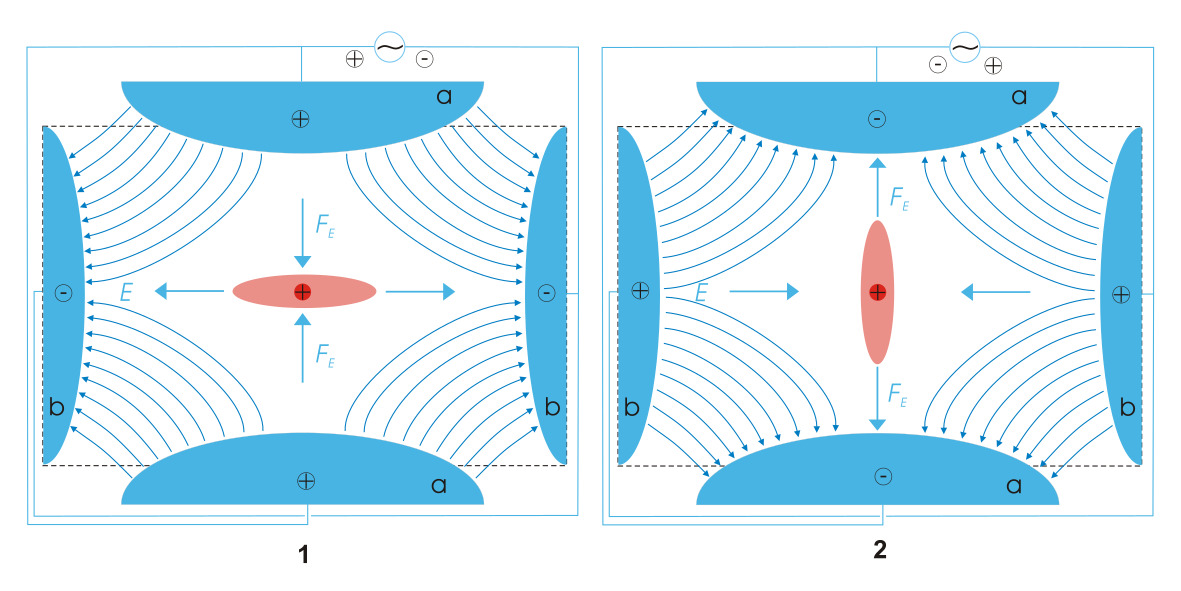
\includegraphics[width=\columnwidth]{fig/Paul-Trap.png}
    \caption{Paul Trap}
    \label{fig:Paul_Trap}
\end{figure}

Lasers are then used to manipulate the energy states of the electrons. These qubits are promising because of their stability, making them relatively easy to manipulate. However, they are challenging to produce and operate at scale. Companies such as Pasqal and QuEra (\cite{wintersperger_neutral_2023}, \cite{noauthor_building_nodate}) have developed quantum computers based on this technology, particularly using Rydberg atoms. These hydrogen-like atoms have electrons in highly excited states, making them highly sensitive to electromagnetic fields and conducive to entanglement.

The Hamiltonian of a Rydberg atom is expressed as:

\begin{equation}
\hat{H}_0 = -\frac{\hbar^2}{2m}\nabla^2 - \frac{e^2}{4\pi\epsilon_0 r}
\end{equation}


where \( m \) is the electron’s mass, \( \hbar \) is the reduced Planck constant, \( e \) is the electron charge, \( \epsilon_0 \) is the permittivity of free space, and \( r \) is the electron’s distance from the nucleus.

Focusing on two energy levels, denoted \( |g\rangle \) (ground) and \( |e\rangle \) (excited), the reduced Hamiltonian matrix becomes:

\begin{equation}
\hat{H} = \begin{pmatrix}
E_g & \Omega/2 \\
\Omega/2 & E_e
\end{pmatrix}
\end{equation}


where \( E_g \) and \( E_e \) are the energy levels, and \( \Omega \) represents the Rabi frequency, proportional to the applied electromagnetic field.

This simplified form omits the complexity of interactions between multiple electrons and coupling with electromagnetic fields. Nonetheless, it highlights the physical basis for using Rydberg atoms as qubits.

% \subsection{Superconducting qubits}

% Superconducting qubits are created using electrical circuits cooled to extremely low temperatures to achieve superconductivity. At these temperatures, resistance vanishes due to the formation of Cooper pairs (pairs of electrons behaving as bosons). These pairs allow a collective quantum state to form, enabling qubit manipulation.

% Consider an LC circuit, where \( L \) is the inductance and \( C \) the capacitance:

% \begin{figure}[H]
%     \centering
%     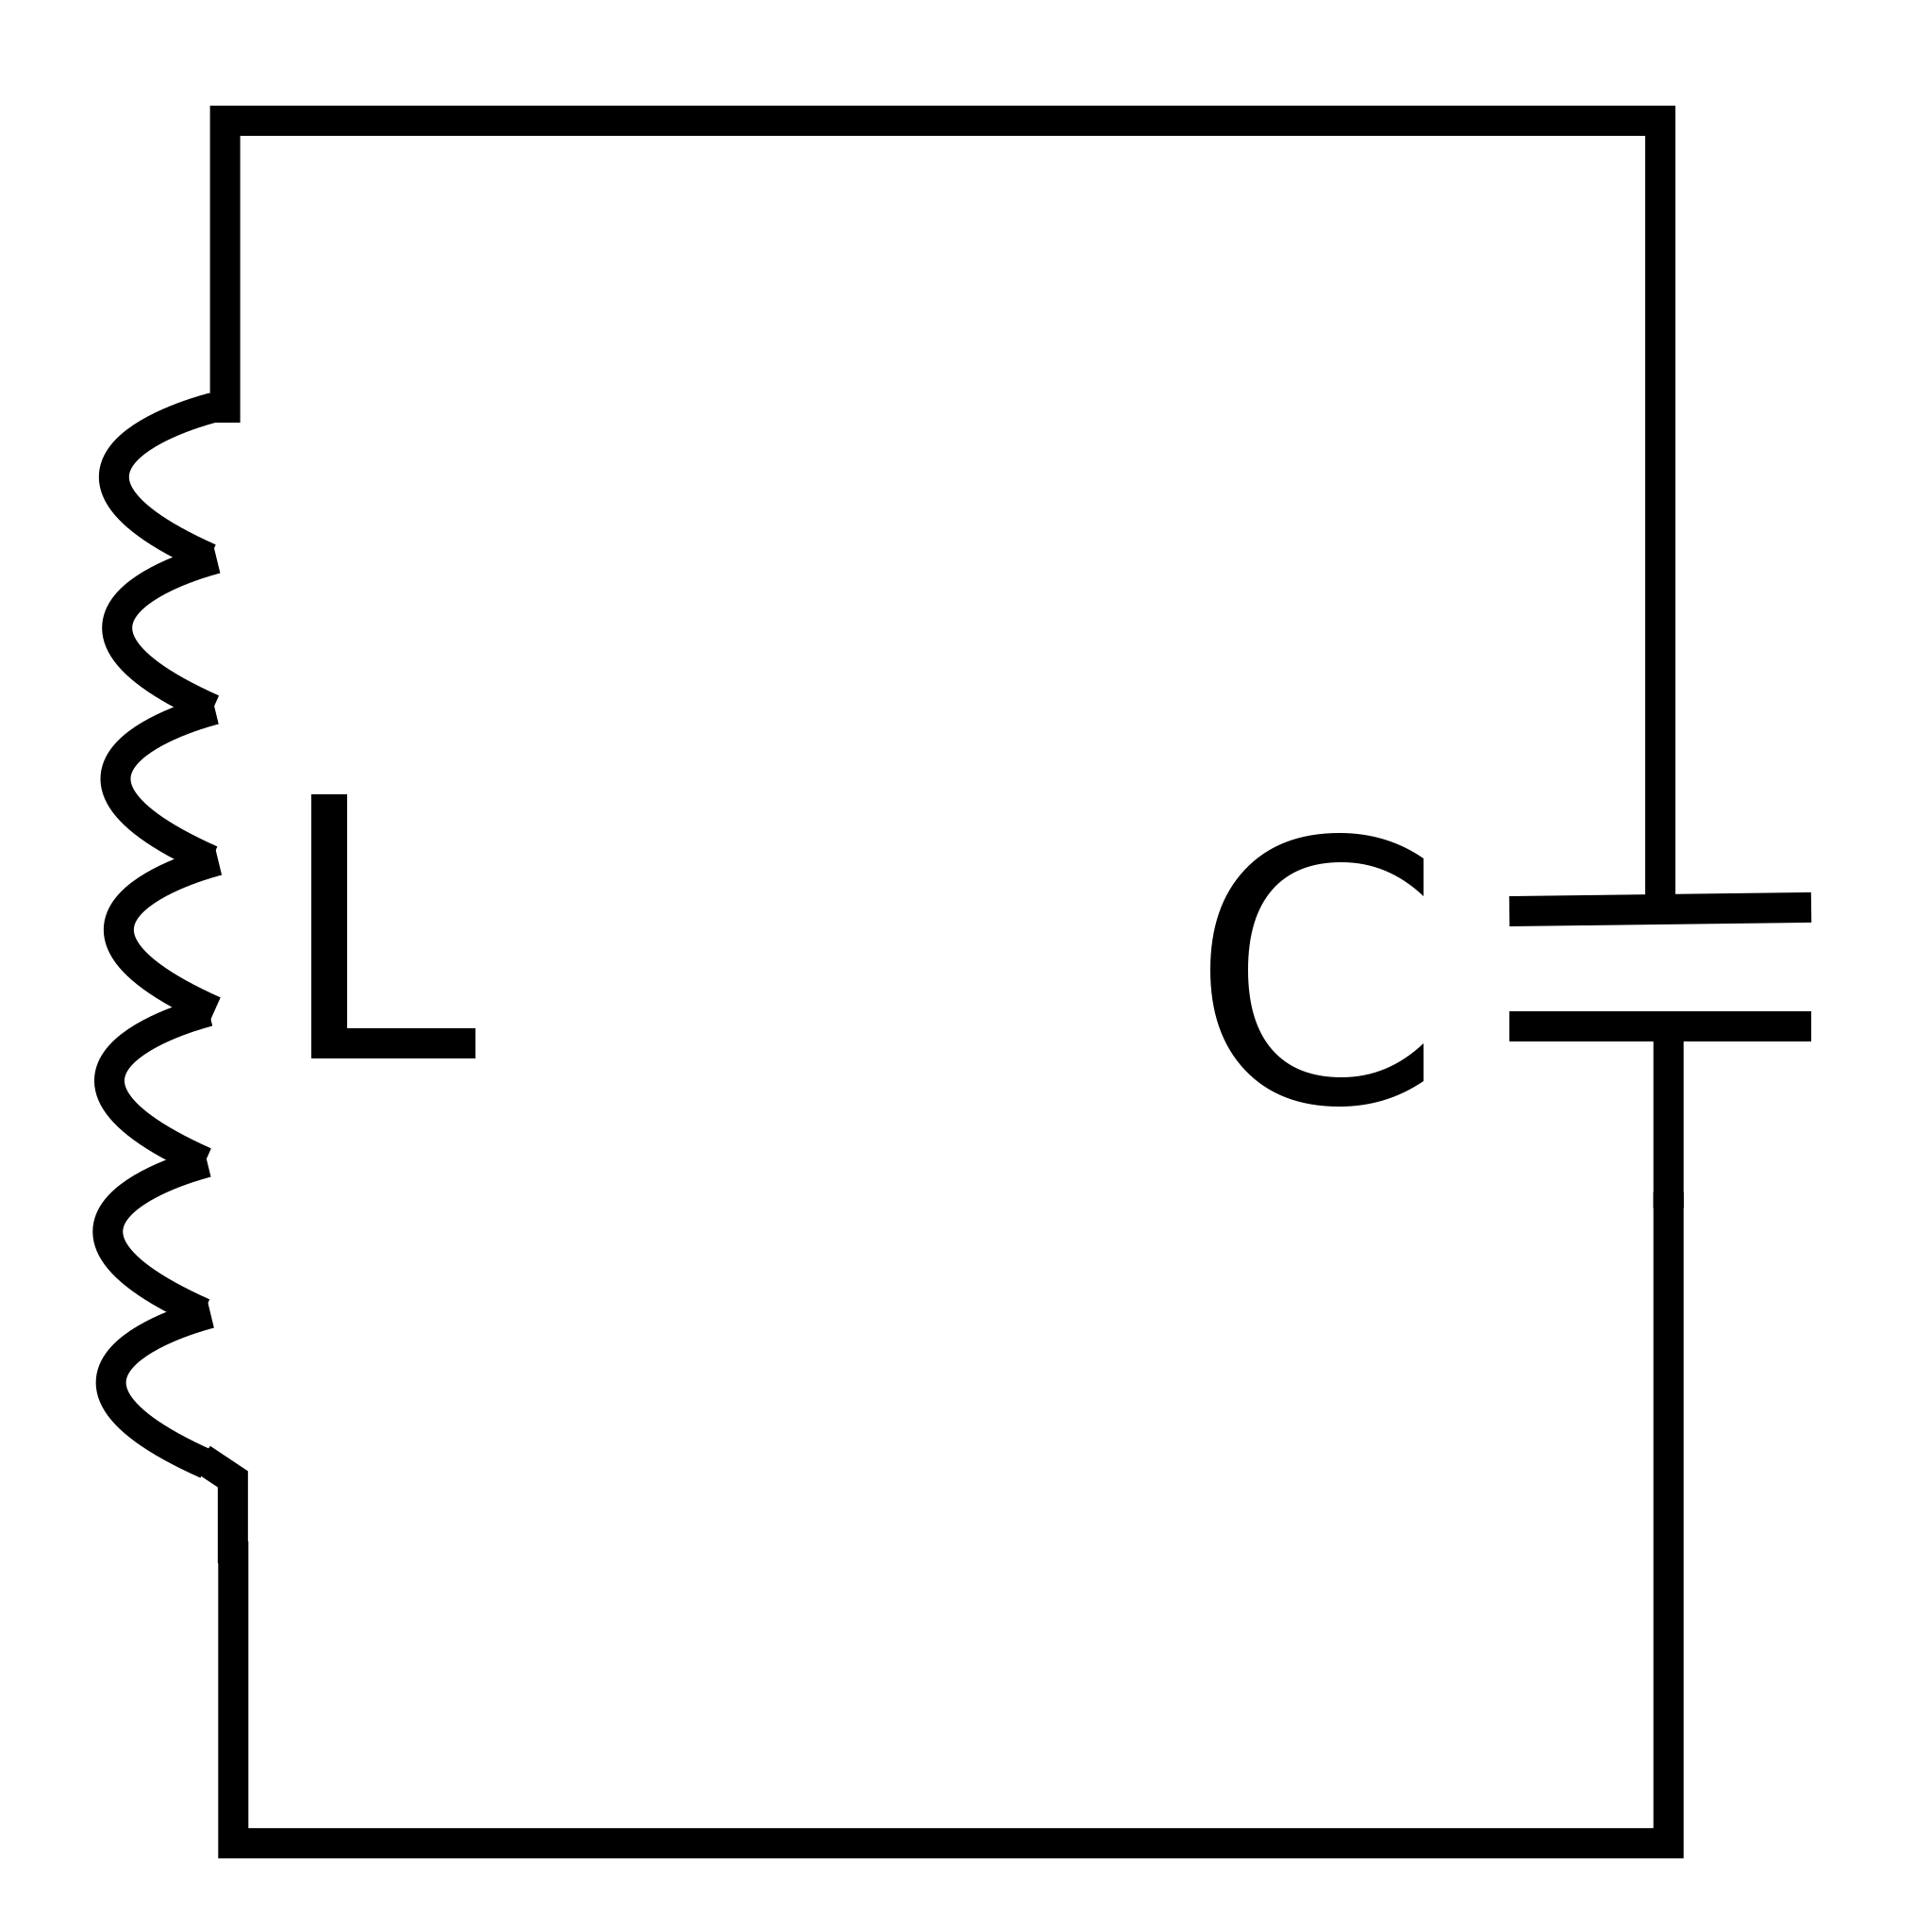
\includegraphics[width=0.7\columnwidth]{fig/circuit_LC.png}
%     \caption{LC Circuit}
%     \label{fig:Circuit_LC}
% \end{figure}

% The Hamiltonian of this circuit is given by:

% \[
% H = \frac{\hat{Q}^2}{2C} + \frac{\hat{\Phi}^2}{2L}
% \]

% where \( \hat{Q} \) is the charge operator and \( \hat{\Phi} \) is the flux operator.

% In practice, superconducting quantum computers like those from IBM and Google employ a specialized circuit called a transmon, depicted below:

% \begin{figure}[H]
%     \centering
%     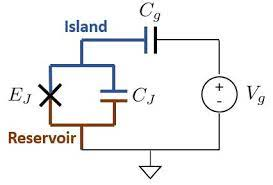
\includegraphics[width=\columnwidth]{fig/transmon_circuit.jpg}
%     \caption{Transmon Circuit}
%     \label{fig:transmon}
% \end{figure}

% The transmon’s Hamiltonian takes the form:

% \[
% H = 4E_c\hat{n}^2 - E_J\cos(\hat{\phi})
% \]

% where \( E_c \) is the charging energy, \( E_J \) the Josephson energy, and \( \hat{n} \) and \( \hat{\phi} \) are the operators for the number of Cooper pairs and the phase across the Josephson junction, respectively.

% This circuit behaves like a quantum harmonic oscillator, with two energy levels used for qubit manipulation. The Josephson effect enables coupling between superconducting qubits, facilitating entanglement.

\subsection{Superconducting Qubits}

Superconducting qubits are electrical circuits cooled to extremely low temperatures to render them superconducting. 
At such temperatures, these circuits lose their electrical resistance, enabled by the formation of Cooper pairs, consisting of two electrons behaving as bosons. 
In these materials, all electrons can potentially form Cooper pairs and share the same quantum state, allowing the creation of qubits without the need for individual atoms.

We consider an LC circuit, where \(L\) is the inductance and \(C\) is the capacitance.

\begin{figure}[H]
    \centering
    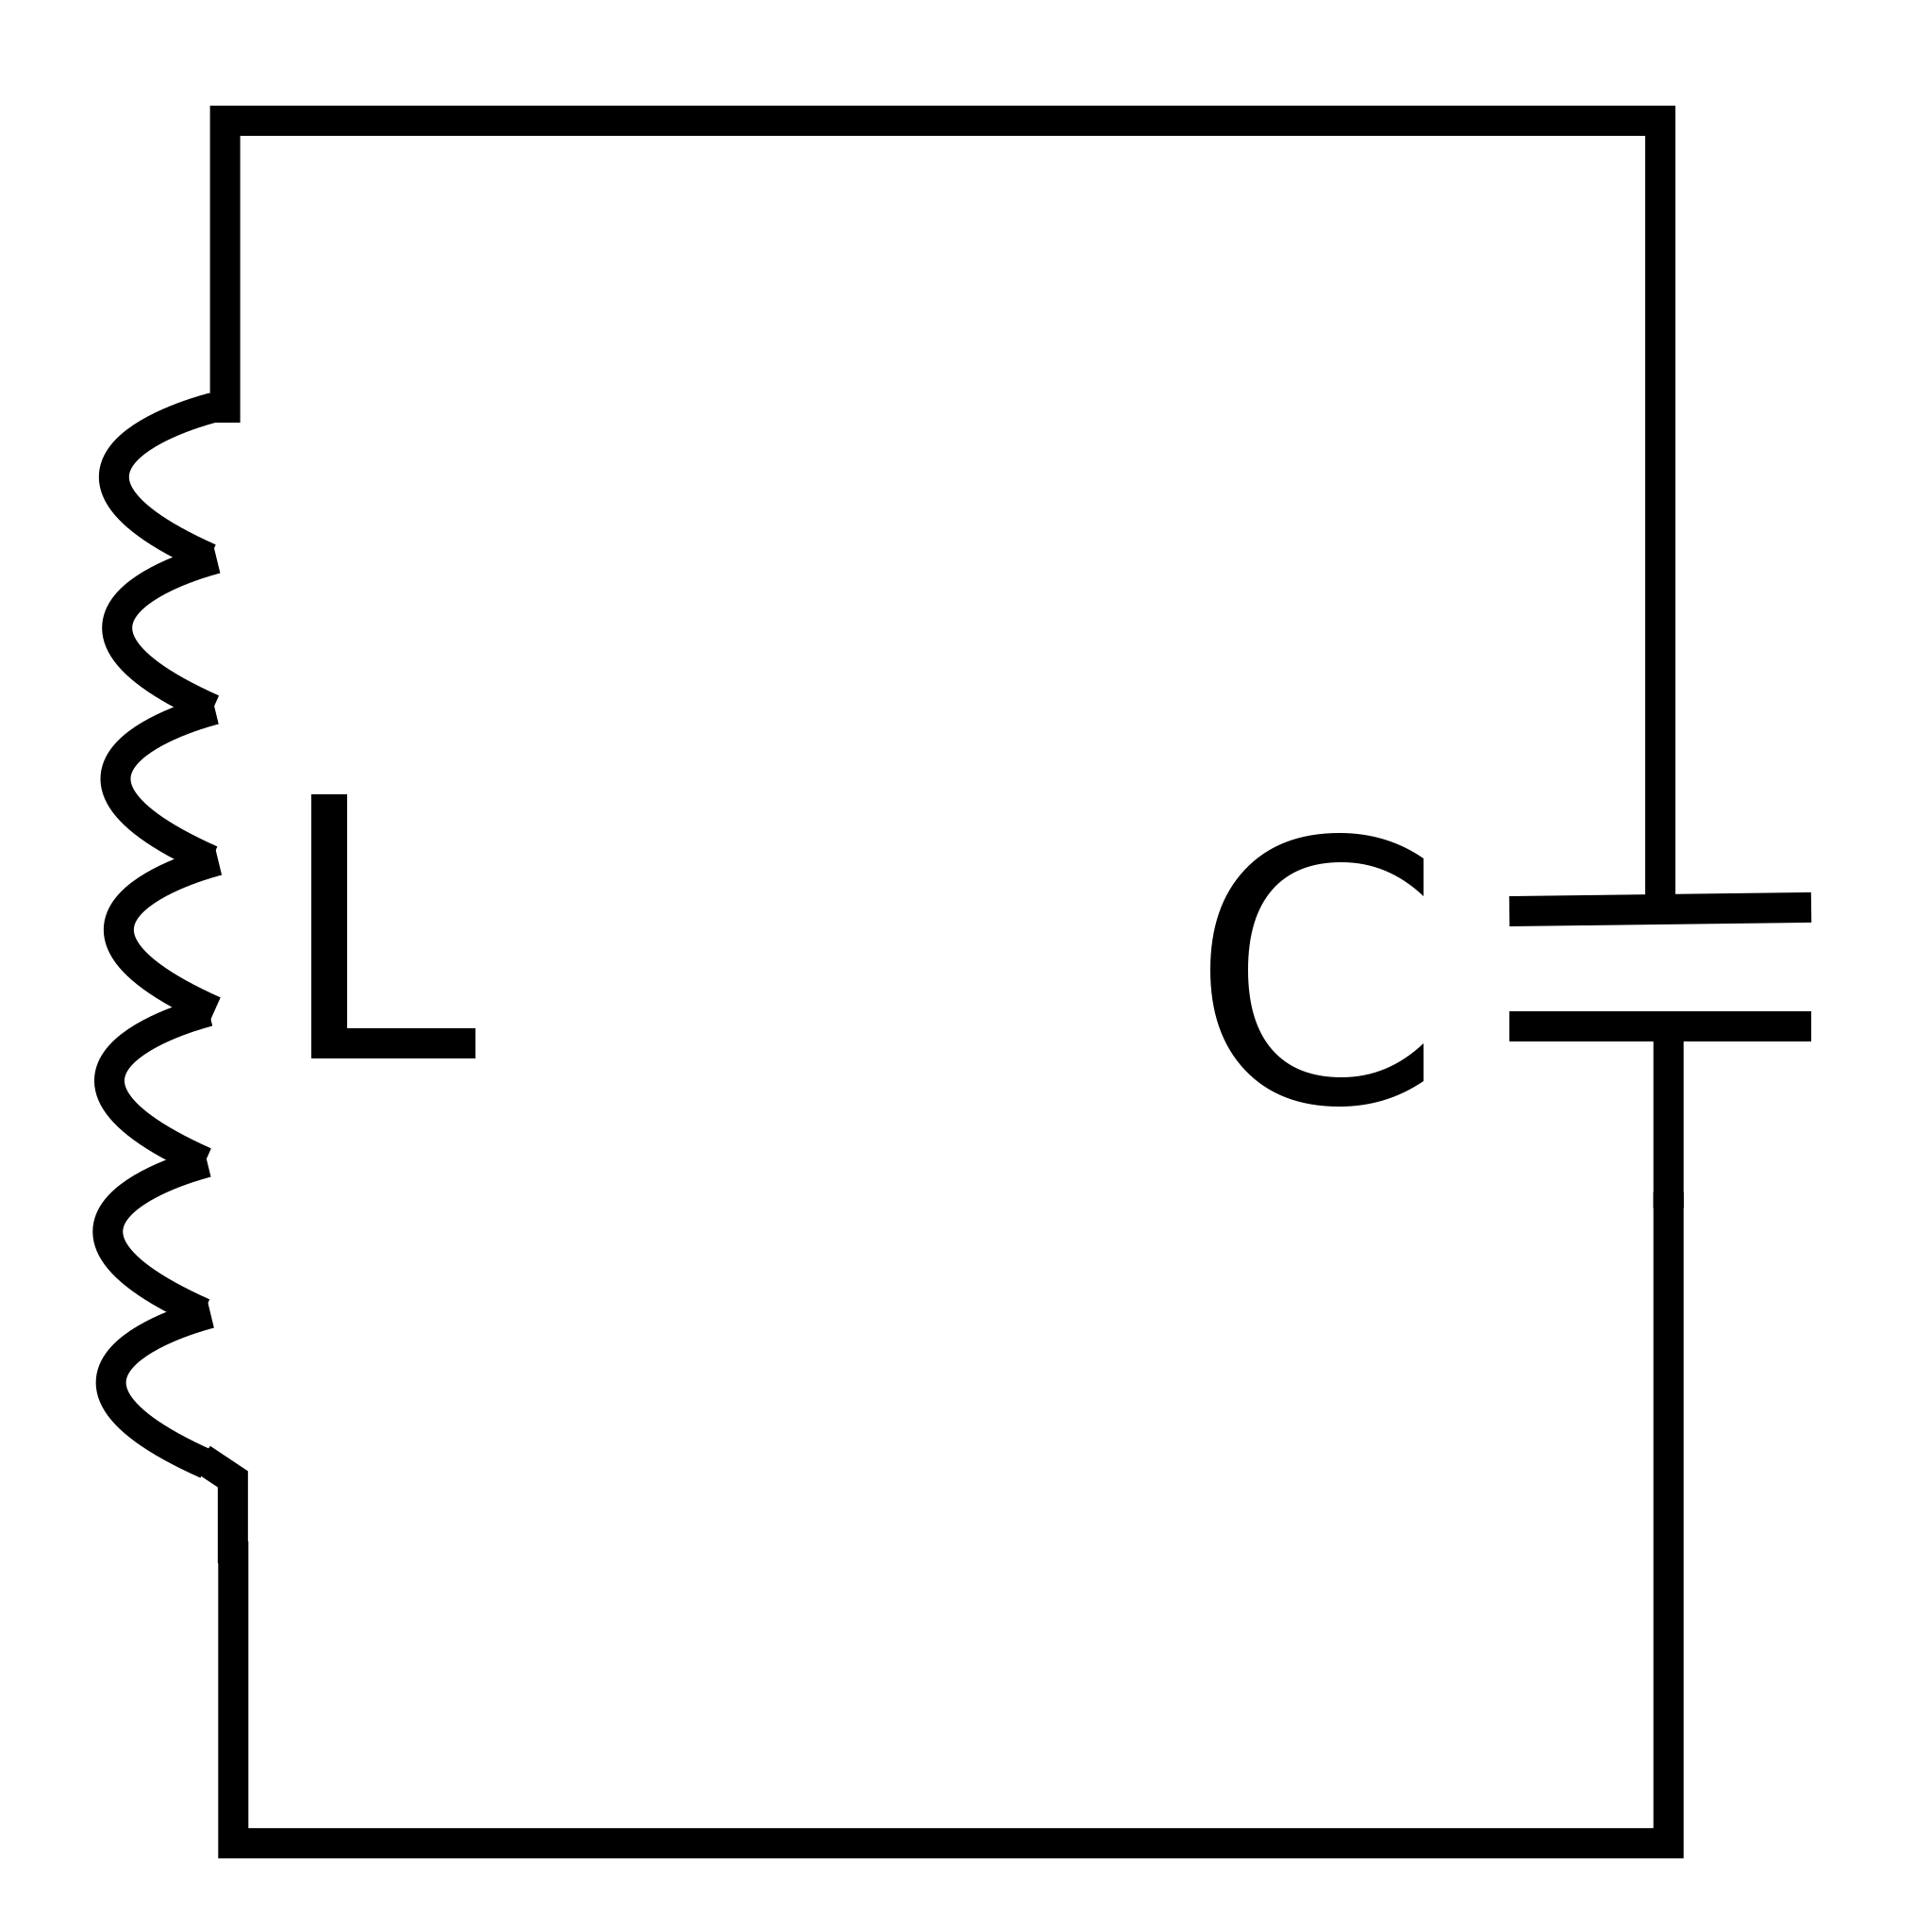
\includegraphics[width = 0.7\columnwidth]{fig/circuit_LC.png}
    \caption{LC Circuit}
    \label{fig:Circuit_LC}
\end{figure}

The Hamiltonian for this circuit can be expressed as follows:

\begin{equation}
H = \frac{{\hat{Q}^2}}{{2C}} + \frac{{\hat{\Phi}^2}}{{2L}}
\end{equation}

The quantized Hamiltonian above is often written in a more convenient form using the reduced charge \(\hat{n} = \hat{Q}/2e\) and the phase \(\hat{\phi} = 2\pi\hat{\Phi}/\Phi_0\), where \(\Phi_0 = h/2e\) is the flux quantum, corresponding to the operators for the number of Cooper pairs and the phase across the Josephson junction, respectively. The quantized Hamiltonian then becomes:

\begin{equation}
H = 4E_c\hat{n}^2 - E_L\frac{d^2}{d\hat{\Phi}^2}
\end{equation}

A qubit is then represented by a portion of material where all electrons share the same quantum state. 
Since electrons behave approximately as harmonic oscillators within the material, it is possible to focus on two energy levels of these oscillators for quantum manipulation.

An interesting aspect is the Josephson effect, which arises from the macroscopic and continuous nature of the wavefunction of Cooper pairs. 
This means that bringing two superconducting boxes close to each other can create a coupling between their wavefunctions, facilitating quantum entanglement.

These circuits behave as quantum oscillators that can exist in two base states. Transistors can be used to act on the state of these oscillators, enabling the production of qubits.

Superconducting quantum computers, such as those produced by IBM and Google, use a specific circuit called a transmon.

\begin{figure}[H]
    \centering
    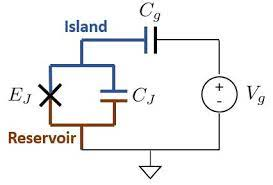
\includegraphics[width = \columnwidth]{fig/transmon_circuit.jpg}
    \caption{Transmon Circuit}
    \label{fig:transmon}
\end{figure}

Without delving into details, this circuit is analogous to an LC circuit (as shown in \autoref{fig:transmon}), where the Hamiltonian is given by:

\begin{equation}
H = 4E_c\hat{n}^2 - E_J\cos(\hat{\phi})
\end{equation}

where \(E_c\) is the charging energy, \(E_J\) is the Josephson energy, and \(\hat{n}\) and \(\hat{\phi}\) are the operators for the number of Cooper pairs and the phase across the Josephson junction, respectively.

Transmons also resemble quantum oscillators, as shown in the figure representing their energy levels (from IBM documentation \cite{noauthor_introduction_nodate}):

\begin{figure}[H]
    \centering
    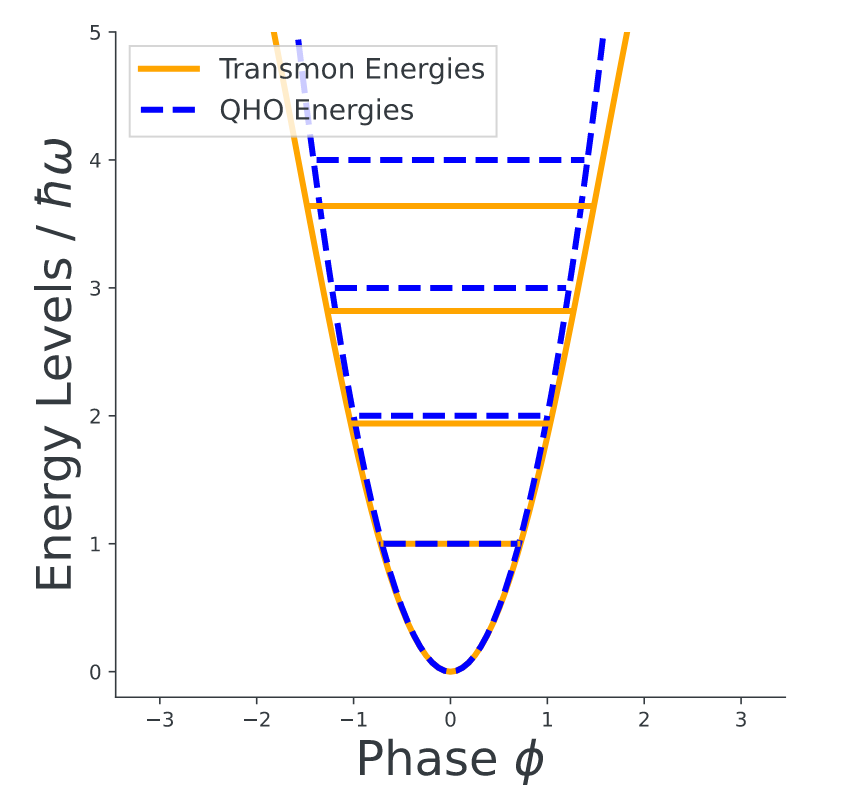
\includegraphics[width = \columnwidth]{fig/transfon.png}
    \caption{Energy levels of a Transmon (IBM)}
    \label{fig:Transmon}
\end{figure}

\subsection{Photonic qubits}

A straightforward and intuitive way to create qubits is using photons. Photon polarization can be decomposed into two basis states, denoted \( \left|0\right> \) and \( \left|1\right> \). Optical fibers and devices such as polarizers are used to manipulate the state of photonic qubits.

\begin{figure}[H]
    \centering
    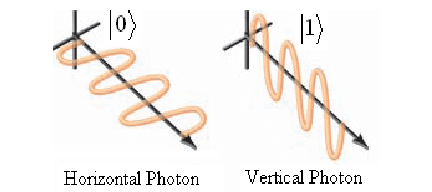
\includegraphics[width=\columnwidth]{fig/Single-photon-qubit.png}
    \caption{Photonic Qubit}
    \label{fig:Qubit_a_photons}
\end{figure}

Unlike other technologies, the energy Hamiltonian is not of primary interest for photonic qubits. Instead, operators like \( \hat{\sigma}_z \) measure polarization states and are implemented via polarizing filters.

\subsection{Which technology to choose?}

It is challenging to determine which technology is the most promising. Each has its advantages and disadvantages. IBM, with its superconducting qubits, and Pasqal, with its trapped-ion qubits, appear highly scalable, allowing for a large number of qubits. However, applying logical operations to these qubits can modify the information, such as flipping a qubit from the state \( \left|0\right> \) to \( \left|1\right> \). Thus, gate fidelity is a critical issue, though companies rarely disclose such details. To mitigate errors, multiple qubits can be used for error correction—a process called quantum error correction.

Pasqal, for instance, still does not allow logical gates on its qubits, and there are other limitations. For example, trapped-ion superconducting qubits allow for entanglement only between neighboring qubits (spatially), making it hard to entangle distant qubits. Other companies take different approaches, such as Alice & Bob, which focus on cat qubits immune to specific types of errors.

For quantum gate-based computers, performance can be gauged by two metrics: the fidelity of 2-qubit gates and the number of physical qubits. Achieving the NISQ (Noisy Intermediate-Scale Quantum) stage—a key milestone—requires over 40 physical qubits and 2-qubit gate fidelities exceeding 99.9\%. The figure below (\autoref{fig:nisq}) from \cite{ezratty_where_2023} visualizes the performance of various technologies based on the number of qubits and gate fidelities.

\begin{figure}[H]
    \centering
    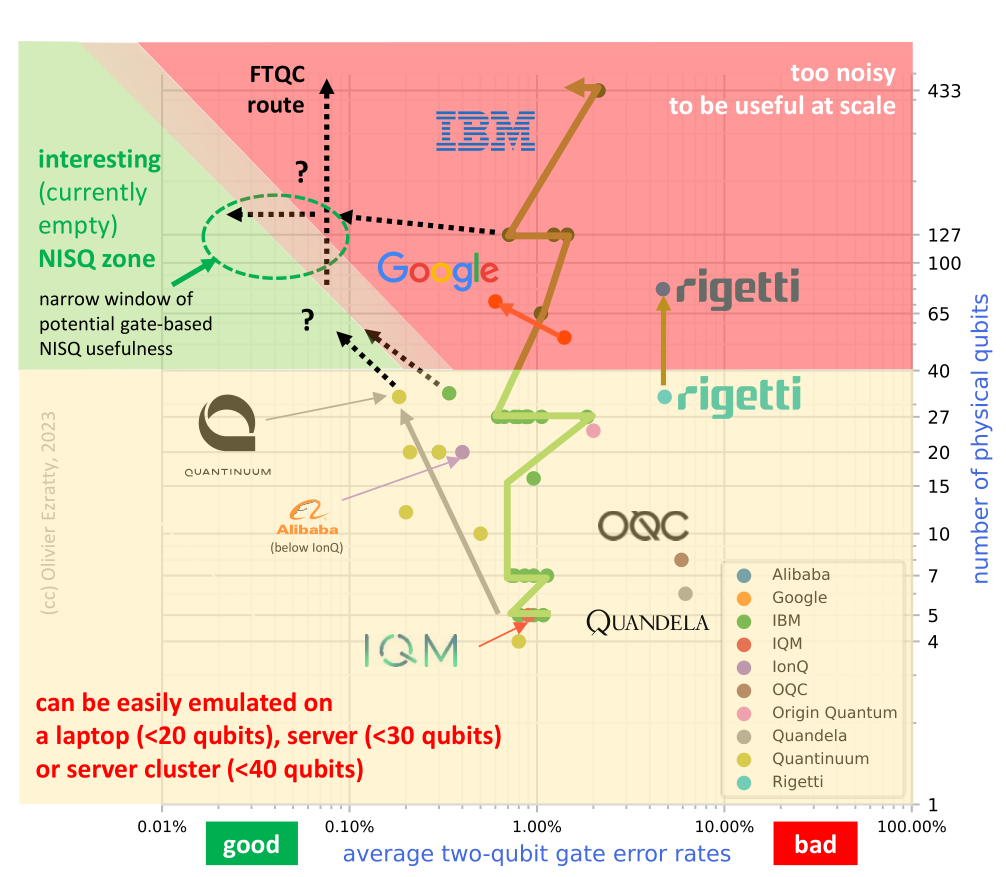
\includegraphics[width = \columnwidth]{fig/NISQ.png}
    \caption{Performance of different technologies by qubit count and 2-qubit gate fidelity}
    \label{fig:nisq}
\end{figure}

To date, the most advanced technology is superconducting qubits, with IBM and Google producing quantum computers exceeding 50 qubits. While gate fidelities are not exceptionally high, IBM provides a variety of gates and highly effective error-correcting codes (\cite{bravyi_high-threshold_2024}).

On the other hand, trapped-ion qubits offer the most promising scalability. Experiments have demonstrated the ability to maintain chains of thousands of these ions, and Quantinuum’s efforts to deliver highly stable qubits are particularly encouraging.

Recent developments by Quantinuum and Microsoft have introduced new error-correcting codes that reduce errors by a factor of 800 (\cite{zander_advancing_2024}), positioning Quantinuum as a potential leader in quantum computing.

It is worth noting that no two quantum computers are identical. Cat qubits are immune to certain errors, trapped-ion qubits exhibit unique physical properties like the Rydberg blockade, and photonic quantum computers operate very differently, offering specialized advantages for specific applications.

\section{Algorithms and Quantum Optimization}

% To manipulate the state of a qubit, we use operators. These operators represent the action of physical measurements on a qubit's state. However, when focusing only on the variables defining a qubit’s state (coefficients \( a \) and \( b \)), the underlying physical system becomes less relevant. Whether we use a Rydberg atom, a superconducting circuit, or a photon, operators can act on the qubit's state similarly, e.g., flipping \( \left|0\right> \) to \( \left|1\right> \) and vice versa.

% \subsection{Quantum gates}

% Quantum gates are the algebraic representations of operators acting on a qubit’s state.

% \section{Manipulating Qubit States}

To manipulate the state of a qubit, we use operators. These operators mathematically represent the effects of physical processes or measurements on a qubit's state. When focusing solely on the abstract mathematical description of the state (defined by the coefficients \(a\) and \(b\) in \(|\psi\rangle = a|0\rangle + b|1\rangle\)), the specific physical realization of the qubit becomes less relevant. Whether the qubit is implemented using a Rydberg atom, a superconducting circuit, or a photon, the same operators can be applied to manipulate the qubit state, such as flipping \(|0\rangle\) to \(|1\rangle\) and vice versa.

\subsection{Quantum Gates}

Quantum gates are the algebraic representations of operators acting on a qubit's state. These gates perform specific transformations, such as rotations or state flips, and are fundamental building blocks in quantum algorithms. Their physical implementation depends on the underlying quantum hardware.

\subsubsection{Pauli gates}

Pauli gates act on a qubit’s state by rotating it about the \( x \), \( y \), or \( z \)-axes. They are defined as follows:

\begin{equation}
    X = \begin{pmatrix} 0 & 1 \\ 1 & 0 \end{pmatrix}
\end{equation}

\begin{equation}
    Y = \begin{pmatrix} 0 & -i \\ i & 0 \end{pmatrix}
\end{equation}

\begin{equation}
    Z = \begin{pmatrix} 1 & 0 \\ 0 & -1 \end{pmatrix}
\end{equation}

\subsubsection{Hadamard gate}

The Hadamard gate rotates a qubit about both the \( x \)- and \( z \)-axes:

\begin{equation}
    H = \frac{1}{\sqrt{2}}\begin{pmatrix} 1 & 1 \\ 1 & -1 \end{pmatrix}
\end{equation}

\subsubsection{Phase gate}

The phase gate rotates a qubit about the \( z \)-axis:

\begin{equation}
    S = \begin{pmatrix} 1 & 0 \\ 0 & i \end{pmatrix}
\end{equation}

\subsubsection{CNOT gate}

The CNOT gate acts on two qubits by flipping the second qubit based on the state of the first qubit:

\begin{equation}
    CNOT = \begin{pmatrix} 1 & 0 & 0 & 0 \\ 0 & 1 & 0 & 0 \\ 0 & 0 & 0 & 1 \\ 0 & 0 & 1 & 0 \end{pmatrix}
\end{equation}

These fundamental gates, when combined, allow for any logical operation to be performed on the states of qubits.

\subsection{Quantum optimization}

One significant application of quantum properties is solving optimization problems. If we can encode an optimization problem’s cost into the Hamiltonian of a quantum system, finding the ground state of that system corresponds to solving the optimization problem.

\subsubsection{Adiabatic theorem}

To find the ground state of a quantum system, we rely on the adiabatic theorem. This theorem states that if a quantum system starts in the ground state of its Hamiltonian, and the Hamiltonian changes slowly, the system will remain in the ground state of the Hamiltonian.

Mathematically, if \( \hat{H}(t) \) is the system’s Hamiltonian at time \( t \), and it evolves as:

\begin{equation}
    \hat{H}(t) = (1 - t/T)\hat{H}_0 + (t/T)\hat{H}_f
\end{equation}

where \( \hat{H}_0 \) is the initial Hamiltonian and \( \hat{H}_f \) is the final Hamiltonian at \( t = T \), then for sufficiently large \( T \), the ground state of \( \hat{H}_0 \) evolves into the ground state of \( \hat{H}_f \).

This variation must satisfy the following condition:

\begin{equation}
    \tau \gg \frac{\max_{ 0 \leq s \leq 1}  \left| \left\langle \psi_1(s) \left| \frac{\partial \hat{H}(s)}{\partial s} \right| \psi_0(s) \right\rangle \right| }{\min_{0 \leq s \leq 1} \Delta^2(s)}
\end{equation}

where \( \tau \) is the evolution time, \( \psi_0(s) \) and \( \psi_1(s) \) are the ground and first excited states of the Hamiltonian \( \hat{H}(s) \), and \( \Delta(s) \) is the energy gap between these states.

\subsubsection{Ising Hamiltonian}

To encode our optimization problem, we use the Ising Hamiltonian:

\begin{equation}
    \hat{H} = -\sum_{i,j} J_{ij}\hat{\sigma}_i^z\hat{\sigma}_j^z - \sum_i h_i\hat{\sigma}_i^z
\end{equation}

Here, \( \hat{\sigma}_i^z \) is the Pauli-\( z \) operator, \( J_{ij} \) are coupling weights between spins, and \( h_i \) are local magnetic fields.

A critical point is ensuring that the initial Hamiltonian \( \hat{H}_0 \) does not commute with the Ising Hamiltonian. Otherwise, the initial state would remain stationary for both Hamiltonians, preventing evolution.

\subsection{Optimization problem: Max-Cut}

The Max-Cut problem is a combinatorial optimization task that involves dividing a graph into two subsets to maximize the number of edges crossing between them. The input consists of the graph's nodes and edges. It is categorized as NP-Hard, meaning classical algorithms solve it in exponential time. However, a quantum computer can solve this problem more efficiently.

\begin{figure}[H]
    \centering
    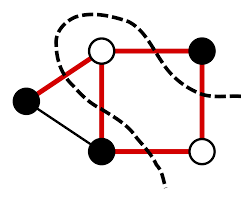
\includegraphics[width = \columnwidth]{fig/Max_Cut.png}
    \caption{Max-Cut problem}
    \label{fig:Max_cut_edge}
\end{figure}

For example, consider a graph with two nodes:

\begin{figure}[H]
    \centering
    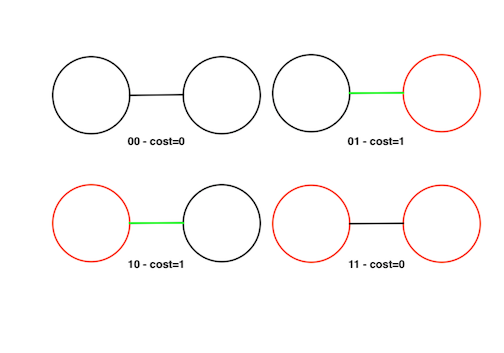
\includegraphics[width = \columnwidth]{fig/02_2_nodes_cuts.png}
    \caption{Max-Cut with 2 nodes}
    \label{fig:Max_cut_edge_2}
\end{figure}

Here is another example with three nodes:

\begin{figure}[H]
    \centering
    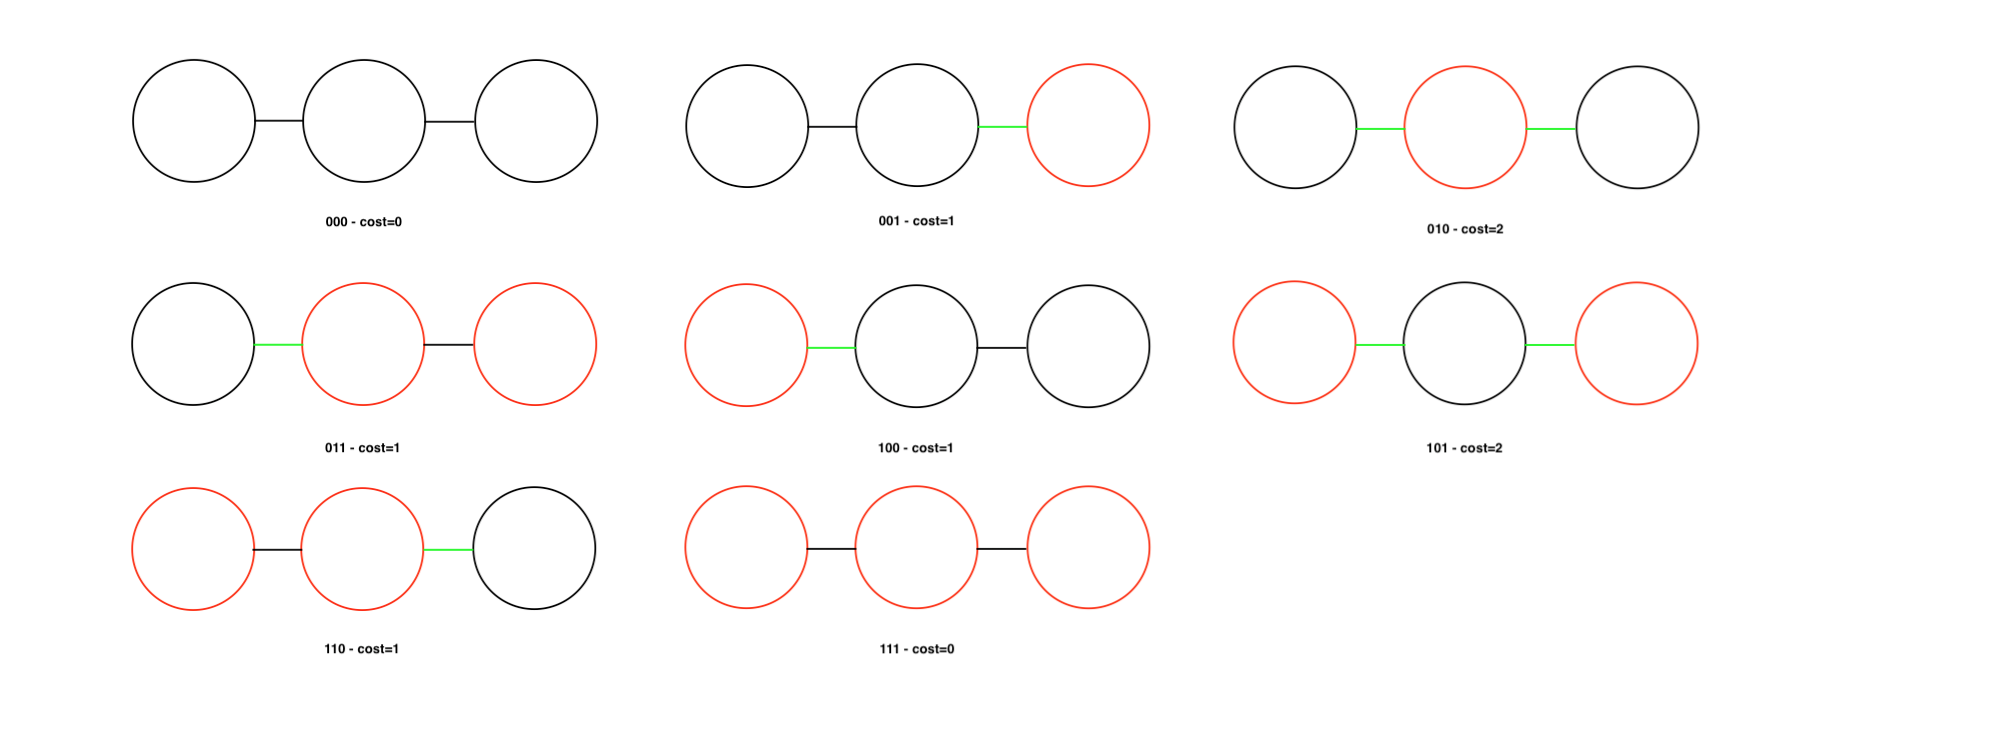
\includegraphics[width = \columnwidth]{fig/02_3_nodes_cuts.png}
    \caption{Max-Cut with 3 nodes}
    \label{fig:Max_cut_edge_3}
\end{figure}

The cost function for the problem can be expressed as:

\begin{equation}
    C_{total} = \sum C_{ij} = \sum \frac{1}{2} w_{ij} (1 - z_i z_j)
\end{equation}

where \( w_{ij} = 1 \) if \( i \) and \( j \) are connected by an edge, \( 0 \) otherwise. The binary variables \( z_i \) and \( z_j \) define whether a node belongs to one of the subsets.

\subsection{Quantum encoding of the problem: Which Hamiltonian?}

The Max-Cut problem is well-suited for encoding into an Ising Hamiltonian. Each node of the graph corresponds to a qubit, and coupling weights are assigned between qubits if their respective nodes are connected by an edge.

The Ising Hamiltonian is then defined as:

\begin{equation}
    \hat{H} = -\sum_{i,j} J_{ij}\hat{\sigma}_i^z\hat{\sigma}_j^z - \sum_i h_i\hat{\sigma}_i^z
\end{equation}

with coupling weights:

\begin{equation}
    J_{ij} = \begin{cases} 
    1 & \text{if } i \text{ and } j \text{ are connected by an edge} \\
    0 & \text{otherwise}
    \end{cases}
\end{equation}

and local magnetic fields:

\begin{equation}
    h_i = 0
\end{equation}

The state of each qubit (\( \left|0\right> \) or \( \left|1\right> \)) determines its subset, avoiding the need for additional qubits to encode this information (as in classical bits).

\subsection{Implementation}

To solve the Max-Cut problem, we use the Leap library to encode the problem and execute it on a D-Wave quantum annealer. D-Wave devices specialize in quantum annealing, allowing us to define the Hamiltonian for our qubits without implementing logical gates.

The code below, based on prior work (\cite{jain_solving_2021}, \cite{stechly_mstechlyquantum_tsp_tutorials_2024}), first formulates the problem as a graph:

\begin{lstlisting}[language=Python]
    G = nx.Graph()
    G.add_edges_from([
        [0,3],[0,4],[1,3],[1,4],
        [2,3],[2,4],[3,5],[1,3],
        [6,7], [2,7], [5,7], [3,5]
    ])
    nx.draw(G, 
        pos=nx.bipartite_layout(
            G, [0,1,2]
        ))
\end{lstlisting}

This produces the following graph:

\begin{figure}[H]
    \centering
    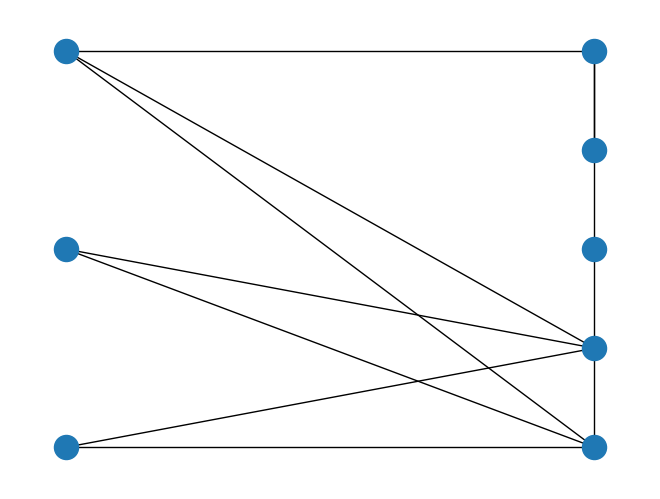
\includegraphics[width = \columnwidth]{fig/oriented_graph.png}
    \caption{Graph for the problem}
    \label{fig:Graph_problem}
\end{figure}

The graph is then converted into an Ising Hamiltonian:

\begin{lstlisting}[language=Python]
    # Initialize h vector and J matrix
    h = defaultdict(int)
    J = defaultdict(int)

    # Update J matrix for each edge in the graph
    for i, j in G.edges:
        J[(i,j)] += 1
\end{lstlisting}

A sampler instance, corresponding to the quantum computer, is created:

\begin{lstlisting}[language=Python]
    # Initialize quantum sampler
    client = Client.from_config(
        config_file="dwave.conf",
        profile="bqm"
    )
    sampler = EmbeddingComposite(
        DWaveSampler()
    )
    
    # Define parameters
    chainstrength = 2
    numruns = 10
\end{lstlisting}

Finally, the Hamiltonian is submitted to the sampler, which returns the optimized solution:

\begin{lstlisting}[language=Python]
    # Solve the problem
    response = sampler.sample_ising(h, J) 
\end{lstlisting}

The solution is presented as follows:

\begin{table}[H]
    \centering
    \begin{tabular}{cccccccc}
        \hline
        0 & 1 & 2 & 3 & 4 & 5 & 6 & 7 \\
        \hline
        -1 & -1 & -1 & +1 & +1 & -1 & -1 & +1 \\
        +1 & +1 & +1 & -1 & -1 & +1 & +1 & -1 \\
    \end{tabular}
    \caption{Maximum cut solution for the graph}
    \label{tab:Solution}
\end{table}

The solution can be visualized as follows:

\begin{figure}[H]
    \centering
    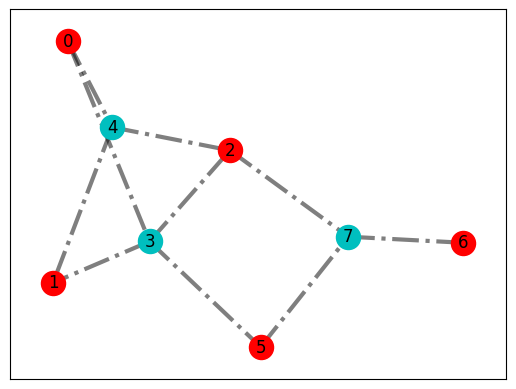
\includegraphics[width = \columnwidth]{fig/solution.png}
    \caption{Visualization of the maximum cut solution}
    \label{fig:Graph_solution}
\end{figure}

\section{Conclusion}

This bibliographic project introduced the fundamental principles of quantum computing, particularly the concept of qubits, methods for producing them, and associated challenges. It also demonstrated solving a classical optimization problem, the Max-Cut, using a quantum computer.

Qubits, with their unique properties like superposition and entanglement, enable computations far more efficient than classical bits. However, their manipulation remains delicate due to the irreversible nature of measurement.

We discussed several technologies for producing qubits, such as superconducting qubits, trapped-ion qubits, and photonic qubits, each with its strengths and weaknesses.

Finally, the project explored solving the Max-Cut problem using quantum annealing, showcasing how quantum computers can encode and optimize problems efficiently. As quantum computing continues to develop, it holds immense promise for addressing complex computational challenges.

\printbibliography

\end{multicols}

\end{document}
